\documentclass[1p]{elsarticle_modified}
%\bibliographystyle{elsarticle-num}

%\usepackage[colorlinks]{hyperref}
%\usepackage{abbrmath_seonhwa} %\Abb, \Ascr, \Acal ,\Abf, \Afrak
\usepackage{amsfonts}
\usepackage{amssymb}
\usepackage{amsmath}
\usepackage{amsthm}
\usepackage{scalefnt}
\usepackage{amsbsy}
\usepackage{kotex}
\usepackage{caption}
\usepackage{subfig}
\usepackage{color}
\usepackage{graphicx}
\usepackage{xcolor} %% white, black, red, green, blue, cyan, magenta, yellow
\usepackage{float}
\usepackage{setspace}
\usepackage{hyperref}

\usepackage{tikz}
\usetikzlibrary{arrows}

\usepackage{multirow}
\usepackage{array} % fixed length table
\usepackage{hhline}

%%%%%%%%%%%%%%%%%%%%%
\makeatletter
\renewcommand*\env@matrix[1][\arraystretch]{%
	\edef\arraystretch{#1}%
	\hskip -\arraycolsep
	\let\@ifnextchar\new@ifnextchar
	\array{*\c@MaxMatrixCols c}}
\makeatother %https://tex.stackexchange.com/questions/14071/how-can-i-increase-the-line-spacing-in-a-matrix
%%%%%%%%%%%%%%%

\usepackage[normalem]{ulem}

\newcommand{\msout}[1]{\ifmmode\text{\sout{\ensuremath{#1}}}\else\sout{#1}\fi}
%SOURCE: \msout is \stkout macro in https://tex.stackexchange.com/questions/20609/strikeout-in-math-mode

\newcommand{\cancel}[1]{
	\ifmmode
	{\color{red}\msout{#1}}
	\else
	{\color{red}\sout{#1}}
	\fi
}

\newcommand{\add}[1]{
	{\color{blue}\uwave{#1}}
}

\newcommand{\replace}[2]{
	\ifmmode
	{\color{red}\msout{#1}}{\color{blue}\uwave{#2}}
	\else
	{\color{red}\sout{#1}}{\color{blue}\uwave{#2}}
	\fi
}

\newcommand{\Sol}{\mathcal{S}} %segment
\newcommand{\D}{D} %diagram
\newcommand{\A}{\mathcal{A}} %arc


%%%%%%%%%%%%%%%%%%%%%%%%%%%%%5 test

\def\sl{\operatorname{\textup{SL}}(2,\Cbb)}
\def\psl{\operatorname{\textup{PSL}}(2,\Cbb)}
\def\quan{\mkern 1mu \triangleright \mkern 1mu}

\theoremstyle{definition}
\newtheorem{thm}{Theorem}[section]
\newtheorem{prop}[thm]{Proposition}
\newtheorem{lem}[thm]{Lemma}
\newtheorem{ques}[thm]{Question}
\newtheorem{cor}[thm]{Corollary}
\newtheorem{defn}[thm]{Definition}
\newtheorem{exam}[thm]{Example}
\newtheorem{rmk}[thm]{Remark}
\newtheorem{alg}[thm]{Algorithm}

\newcommand{\I}{\sqrt{-1}}
\begin{document}

%\begin{frontmatter}
%
%\title{Boundary parabolic representations of knots up to 8 crossings}
%
%%% Group authors per affiliation:
%\author{Yunhi Cho} 
%\address{Department of Mathematics, University of Seoul, Seoul, Korea}
%\ead{yhcho@uos.ac.kr}
%
%
%\author{Seonhwa Kim} %\fnref{s_kim}}
%\address{Center for Geometry and Physics, Institute for Basic Science, Pohang, 37673, Korea}
%\ead{ryeona17@ibs.re.kr}
%
%\author{Hyuk Kim}
%\address{Department of Mathematical Sciences, Seoul National University, Seoul 08826, Korea}
%\ead{hyukkim@snu.ac.kr}
%
%\author{Seokbeom Yoon}
%\address{Department of Mathematical Sciences, Seoul National University, Seoul, 08826,  Korea}
%\ead{sbyoon15@snu.ac.kr}
%
%\begin{abstract}
%We find all boundary parabolic representation of knots up to 8 crossings.
%
%\end{abstract}
%\begin{keyword}
%    \MSC[2010] 57M25 
%\end{keyword}
%
%\end{frontmatter}

%\linenumbers
%\tableofcontents
%
\newcommand\colored[1]{\textcolor{white}{\rule[-0.35ex]{0.8em}{1.4ex}}\kern-0.8em\color{red} #1}%
%\newcommand\colored[1]{\textcolor{white}{ #1}\kern-2.17ex	\textcolor{white}{ #1}\kern-1.81ex	\textcolor{white}{ #1}\kern-2.15ex\color{red}#1	}

{\Large $\underline{12n_{0545}~(K12n_{0545})}$}

\setlength{\tabcolsep}{10pt}
\renewcommand{\arraystretch}{1.6}
\vspace{1cm}\begin{tabular}{m{100pt}>{\centering\arraybackslash}m{274pt}}
\multirow{5}{120pt}{
	\centering
	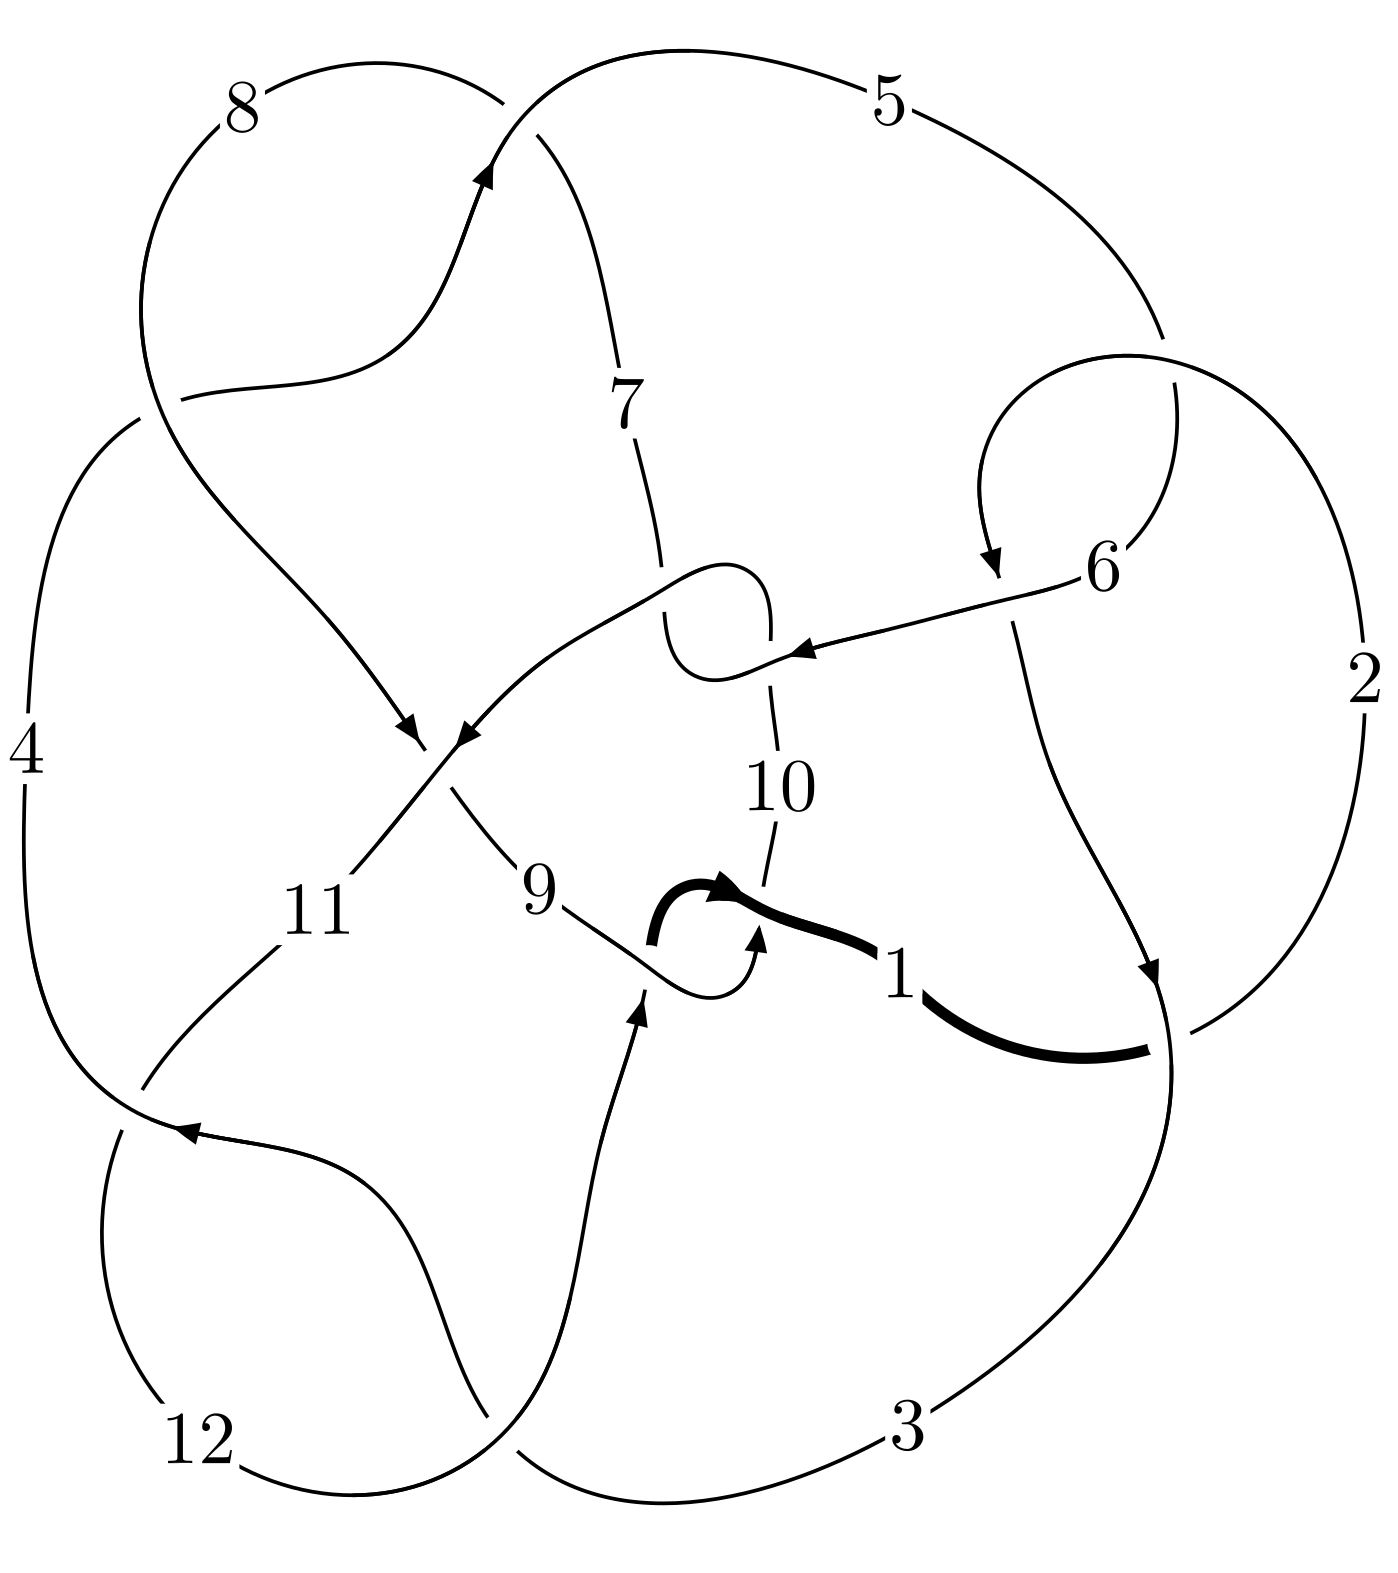
\includegraphics[width=112pt]{../../../GIT/diagram.site/Diagrams/png/2634_12n_0545.png}\\
\ \ \ A knot diagram\footnotemark}&
\allowdisplaybreaks
\textbf{Linearized knot diagam} \\
\cline{2-2}
 &
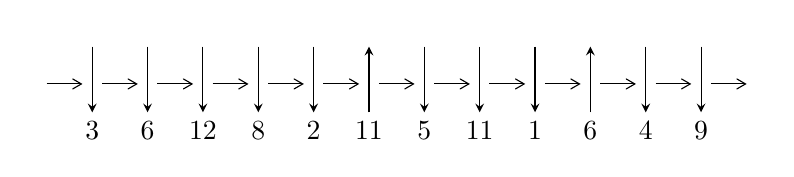
\begin{tikzpicture}[x=20pt, y=17pt]
	% nodes
	\node (C0) at (0, 0) {};
	\node (C1) at (1, 0) {};
	\node (C1U) at (1, +1) {};
	\node (C1D) at (1, -1) {3};

	\node (C2) at (2, 0) {};
	\node (C2U) at (2, +1) {};
	\node (C2D) at (2, -1) {6};

	\node (C3) at (3, 0) {};
	\node (C3U) at (3, +1) {};
	\node (C3D) at (3, -1) {12};

	\node (C4) at (4, 0) {};
	\node (C4U) at (4, +1) {};
	\node (C4D) at (4, -1) {8};

	\node (C5) at (5, 0) {};
	\node (C5U) at (5, +1) {};
	\node (C5D) at (5, -1) {2};

	\node (C6) at (6, 0) {};
	\node (C6U) at (6, +1) {};
	\node (C6D) at (6, -1) {11};

	\node (C7) at (7, 0) {};
	\node (C7U) at (7, +1) {};
	\node (C7D) at (7, -1) {5};

	\node (C8) at (8, 0) {};
	\node (C8U) at (8, +1) {};
	\node (C8D) at (8, -1) {11};

	\node (C9) at (9, 0) {};
	\node (C9U) at (9, +1) {};
	\node (C9D) at (9, -1) {1};

	\node (C10) at (10, 0) {};
	\node (C10U) at (10, +1) {};
	\node (C10D) at (10, -1) {6};

	\node (C11) at (11, 0) {};
	\node (C11U) at (11, +1) {};
	\node (C11D) at (11, -1) {4};

	\node (C12) at (12, 0) {};
	\node (C12U) at (12, +1) {};
	\node (C12D) at (12, -1) {9};
	\node (C13) at (13, 0) {};

	% arrows
	\draw[->,>={angle 60}]
	(C0) edge (C1) (C1) edge (C2) (C2) edge (C3) (C3) edge (C4) (C4) edge (C5) (C5) edge (C6) (C6) edge (C7) (C7) edge (C8) (C8) edge (C9) (C9) edge (C10) (C10) edge (C11) (C11) edge (C12) (C12) edge (C13) ;	\draw[->,>=stealth]
	(C1U) edge (C1D) (C2U) edge (C2D) (C3U) edge (C3D) (C4U) edge (C4D) (C5U) edge (C5D) (C6D) edge (C6U) (C7U) edge (C7D) (C8U) edge (C8D) (C9U) edge (C9D) (C10D) edge (C10U) (C11U) edge (C11D) (C12U) edge (C12D) ;
	\end{tikzpicture} \\
\hhline{~~} \\& 
\textbf{Solving Sequence} \\ \cline{2-2} 
 &
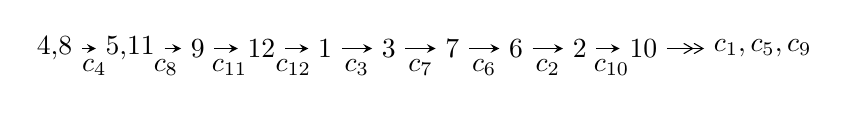
\begin{tikzpicture}[x=23pt, y=7pt]
	% node
	\node (A0) at (-1/8, 0) {4,8};
	\node (A1) at (17/16, 0) {5,11};
	\node (A2) at (17/8, 0) {9};
	\node (A3) at (25/8, 0) {12};
	\node (A4) at (33/8, 0) {1};
	\node (A5) at (41/8, 0) {3};
	\node (A6) at (49/8, 0) {7};
	\node (A7) at (57/8, 0) {6};
	\node (A8) at (65/8, 0) {2};
	\node (A9) at (73/8, 0) {10};
	\node (C1) at (1/2, -1) {$c_{4}$};
	\node (C2) at (13/8, -1) {$c_{8}$};
	\node (C3) at (21/8, -1) {$c_{11}$};
	\node (C4) at (29/8, -1) {$c_{12}$};
	\node (C5) at (37/8, -1) {$c_{3}$};
	\node (C6) at (45/8, -1) {$c_{7}$};
	\node (C7) at (53/8, -1) {$c_{6}$};
	\node (C8) at (61/8, -1) {$c_{2}$};
	\node (C9) at (69/8, -1) {$c_{10}$};
	\node (A10) at (11, 0) {$c_{1},c_{5},c_{9}$};

	% edge
	\draw[->,>=stealth]	
	(A0) edge (A1) (A1) edge (A2) (A2) edge (A3) (A3) edge (A4) (A4) edge (A5) (A5) edge (A6) (A6) edge (A7) (A7) edge (A8) (A8) edge (A9) ;
	\draw[->>,>={angle 60}]	
	(A9) edge (A10);
\end{tikzpicture} \\ 

\end{tabular} \\

\footnotetext{
The image of knot diagram is generated by the software ``\textbf{Draw programme}" developed by Andrew Bartholomew(\url{http://www.layer8.co.uk/maths/draw/index.htm\#Running-draw}), where we modified some parts for our purpose(\url{https://github.com/CATsTAILs/LinksPainter}).
}\phantom \\ \newline 
\centering \textbf{Ideals for irreducible components\footnotemark of $X_{\text{par}}$} 
 
\begin{align*}
I^u_{1}&=\langle 
4.07415\times10^{97} u^{57}-1.87667\times10^{98} u^{56}+\cdots+6.83675\times10^{98} b-3.94295\times10^{98},\\
\phantom{I^u_{1}}&\phantom{= \langle  }-8.87267\times10^{97} u^{57}+3.53450\times10^{98} u^{56}+\cdots+6.83675\times10^{98} a+9.76518\times10^{98},\;u^{58}-4 u^{57}+\cdots+6 u+4\rangle \\
I^u_{2}&=\langle 
-2 u^{15}+6 u^{14}+\cdots+b+1,\\
\phantom{I^u_{2}}&\phantom{= \langle  }- u^{13}+3 u^{12}-10 u^{11}+17 u^{10}-29 u^9+31 u^8-36 u^7+27 u^6-29 u^5+18 u^4-17 u^3+6 u^2+a-3 u,\\
\phantom{I^u_{2}}&\phantom{= \langle  }u^{16}-3 u^{15}+\cdots- u+1\rangle \\
\\
\end{align*}
\raggedright * 2 irreducible components of $\dim_{\mathbb{C}}=0$, with total 74 representations.\\
\footnotetext{All coefficients of polynomials are rational numbers. But the coefficients are sometimes approximated in decimal forms when there is not enough margin.}
\newpage
\renewcommand{\arraystretch}{1}
\centering \section*{I. $I^u_{1}= \langle 4.07\times10^{97} u^{57}-1.88\times10^{98} u^{56}+\cdots+6.84\times10^{98} b-3.94\times10^{98},\;-8.87\times10^{97} u^{57}+3.53\times10^{98} u^{56}+\cdots+6.84\times10^{98} a+9.77\times10^{98},\;u^{58}-4 u^{57}+\cdots+6 u+4 \rangle$}
\flushleft \textbf{(i) Arc colorings}\\
\begin{tabular}{m{7pt} m{180pt} m{7pt} m{180pt} }
\flushright $a_{4}=$&$\begin{pmatrix}1\\0\end{pmatrix}$ \\
\flushright $a_{8}=$&$\begin{pmatrix}0\\u\end{pmatrix}$ \\
\flushright $a_{5}=$&$\begin{pmatrix}1\\u^2\end{pmatrix}$ \\
\flushright $a_{11}=$&$\begin{pmatrix}0.129779 u^{57}-0.516986 u^{56}+\cdots+5.18894 u-1.42834\\-0.0595919 u^{57}+0.274498 u^{56}+\cdots+1.46859 u+0.576728\end{pmatrix}$ \\
\flushright $a_{9}=$&$\begin{pmatrix}-0.00288585 u^{57}+0.0503023 u^{56}+\cdots-2.22480 u-1.52939\\-0.0906534 u^{57}+0.405030 u^{56}+\cdots+1.10469 u+0.502037\end{pmatrix}$ \\
\flushright $a_{12}=$&$\begin{pmatrix}0.189371 u^{57}-0.791484 u^{56}+\cdots+3.72034 u-2.00506\\-0.0595919 u^{57}+0.274498 u^{56}+\cdots+1.46859 u+0.576728\end{pmatrix}$ \\
\flushright $a_{1}=$&$\begin{pmatrix}0.0387990 u^{57}-0.162896 u^{56}+\cdots-3.18685 u-1.73013\\-0.192685 u^{57}+0.853552 u^{56}+\cdots+0.855020 u+1.27477\end{pmatrix}$ \\
\flushright $a_{3}=$&$\begin{pmatrix}-0.296992 u^{57}+0.998359 u^{56}+\cdots-10.6074 u-1.68008\\0.171483 u^{57}-0.586975 u^{56}+\cdots+8.98917 u+2.03171\end{pmatrix}$ \\
\flushright $a_{7}=$&$\begin{pmatrix}u\\u^3+u\end{pmatrix}$ \\
\flushright $a_{6}=$&$\begin{pmatrix}0.0524169 u^{57}-0.224873 u^{56}+\cdots-1.55050 u-2.18646\\-0.174759 u^{57}+0.745226 u^{56}+\cdots+0.209991 u+1.01830\end{pmatrix}$ \\
\flushright $a_{2}=$&$\begin{pmatrix}-0.342530 u^{57}+1.40424 u^{56}+\cdots-3.12486 u+1.77424\\0.141129 u^{57}-0.526127 u^{56}+\cdots+5.69791 u+0.00196869\end{pmatrix}$ \\
\flushright $a_{10}=$&$\begin{pmatrix}-0.103749 u^{57}+0.491535 u^{56}+\cdots+8.67337 u+0.492109\\0.137791 u^{57}-0.597731 u^{56}+\cdots+2.06345 u-1.32119\end{pmatrix}$\\&\end{tabular}
\flushleft \textbf{(ii) Obstruction class $= -1$}\\~\\
\flushleft \textbf{(iii) Cusp Shapes $= 0.123076 u^{57}-0.812943 u^{56}+\cdots-17.7171 u-16.8383$}\\~\\
\newpage\renewcommand{\arraystretch}{1}
\flushleft \textbf{(iv) u-Polynomials at the component}\newline \\
\begin{tabular}{m{50pt}|m{274pt}}
Crossings & \hspace{64pt}u-Polynomials at each crossing \\
\hline $$\begin{aligned}c_{1}\end{aligned}$$&$\begin{aligned}
&u^{58}+41 u^{57}+\cdots-191 u+169
\end{aligned}$\\
\hline $$\begin{aligned}c_{2},c_{5}\end{aligned}$$&$\begin{aligned}
&u^{58}+u^{57}+\cdots-37 u-13
\end{aligned}$\\
\hline $$\begin{aligned}c_{3},c_{11}\end{aligned}$$&$\begin{aligned}
&u^{58}-3 u^{57}+\cdots- u-17
\end{aligned}$\\
\hline $$\begin{aligned}c_{4},c_{7}\end{aligned}$$&$\begin{aligned}
&u^{58}-4 u^{57}+\cdots+6 u+4
\end{aligned}$\\
\hline $$\begin{aligned}c_{6},c_{10}\end{aligned}$$&$\begin{aligned}
&u^{58}+3 u^{57}+\cdots-16568 u+2143
\end{aligned}$\\
\hline $$\begin{aligned}c_{8}\end{aligned}$$&$\begin{aligned}
&u^{58}+u^{57}+\cdots+202 u+3
\end{aligned}$\\
\hline $$\begin{aligned}c_{9},c_{12}\end{aligned}$$&$\begin{aligned}
&u^{58}+3 u^{57}+\cdots+7097 u+431
\end{aligned}$\\
\hline
\end{tabular}\\~\\
\newpage\renewcommand{\arraystretch}{1}
\flushleft \textbf{(v) Riley Polynomials at the component}\newline \\
\begin{tabular}{m{50pt}|m{274pt}}
Crossings & \hspace{64pt}Riley Polynomials at each crossing \\
\hline $$\begin{aligned}c_{1}\end{aligned}$$&$\begin{aligned}
&y^{58}-37 y^{57}+\cdots-1807601 y+28561
\end{aligned}$\\
\hline $$\begin{aligned}c_{2},c_{5}\end{aligned}$$&$\begin{aligned}
&y^{58}-41 y^{57}+\cdots+191 y+169
\end{aligned}$\\
\hline $$\begin{aligned}c_{3},c_{11}\end{aligned}$$&$\begin{aligned}
&y^{58}+47 y^{57}+\cdots-171 y+289
\end{aligned}$\\
\hline $$\begin{aligned}c_{4},c_{7}\end{aligned}$$&$\begin{aligned}
&y^{58}+18 y^{57}+\cdots+356 y+16
\end{aligned}$\\
\hline $$\begin{aligned}c_{6},c_{10}\end{aligned}$$&$\begin{aligned}
&y^{58}+65 y^{57}+\cdots-280143286 y+4592449
\end{aligned}$\\
\hline $$\begin{aligned}c_{8}\end{aligned}$$&$\begin{aligned}
&y^{58}-15 y^{57}+\cdots-60898 y+9
\end{aligned}$\\
\hline $$\begin{aligned}c_{9},c_{12}\end{aligned}$$&$\begin{aligned}
&y^{58}-49 y^{57}+\cdots-11167097 y+185761
\end{aligned}$\\
\hline
\end{tabular}\\~\\
\newpage\flushleft \textbf{(vi) Complex Volumes and Cusp Shapes}
$$\begin{array}{c|c|c}  
\text{Solutions to }I^u_{1}& \I (\text{vol} + \sqrt{-1}CS) & \text{Cusp shape}\\
 \hline 
\begin{aligned}
u &= \phantom{-}0.633756 + 0.791145 I \\
a &= -0.887765 + 0.616824 I \\
b &= -0.553388 + 0.628935 I\end{aligned}
 & -3.87656 - 0.61696 I & -11.92005 - 0.88689 I \\ \hline\begin{aligned}
u &= \phantom{-}0.633756 - 0.791145 I \\
a &= -0.887765 - 0.616824 I \\
b &= -0.553388 - 0.628935 I\end{aligned}
 & -3.87656 + 0.61696 I & -11.92005 + 0.88689 I \\ \hline\begin{aligned}
u &= \phantom{-}0.747067 + 0.601176 I \\
a &= -1.51970 - 0.38331 I \\
b &= -0.401468 - 0.201550 I\end{aligned}
 & -4.20974 - 3.93817 I & -13.2121 + 6.9659 I \\ \hline\begin{aligned}
u &= \phantom{-}0.747067 - 0.601176 I \\
a &= -1.51970 + 0.38331 I \\
b &= -0.401468 + 0.201550 I\end{aligned}
 & -4.20974 + 3.93817 I & -13.2121 - 6.9659 I \\ \hline\begin{aligned}
u &= \phantom{-}0.480297 + 0.959333 I \\
a &= -1.99240 + 0.86576 I \\
b &= -0.172651 - 0.899004 I\end{aligned}
 & -3.54839 - 3.84914 I & -10.22465 + 4.74982 I \\ \hline\begin{aligned}
u &= \phantom{-}0.480297 - 0.959333 I \\
a &= -1.99240 - 0.86576 I \\
b &= -0.172651 + 0.899004 I\end{aligned}
 & -3.54839 + 3.84914 I & -10.22465 - 4.74982 I \\ \hline\begin{aligned}
u &= -0.521709 + 0.983940 I \\
a &= \phantom{-}1.54639 - 0.06752 I \\
b &= \phantom{-}0.506281 - 1.185660 I\end{aligned}
 & \phantom{-}0.09858 + 7.47040 I & -8.00000 - 8.36343 I \\ \hline\begin{aligned}
u &= -0.521709 - 0.983940 I \\
a &= \phantom{-}1.54639 + 0.06752 I \\
b &= \phantom{-}0.506281 + 1.185660 I\end{aligned}
 & \phantom{-}0.09858 - 7.47040 I & -8.00000 + 8.36343 I \\ \hline\begin{aligned}
u &= \phantom{-}0.503661 + 0.728248 I \\
a &= -1.66274 - 0.02895 I \\
b &= -0.391966 - 1.295650 I\end{aligned}
 & \phantom{-}2.85966 - 4.49859 I & -1.23708 + 2.46876 I \\ \hline\begin{aligned}
u &= \phantom{-}0.503661 - 0.728248 I \\
a &= -1.66274 + 0.02895 I \\
b &= -0.391966 + 1.295650 I\end{aligned}
 & \phantom{-}2.85966 + 4.49859 I & -1.23708 - 2.46876 I\\
 \hline 
 \end{array}$$\newpage$$\begin{array}{c|c|c}  
\text{Solutions to }I^u_{1}& \I (\text{vol} + \sqrt{-1}CS) & \text{Cusp shape}\\
 \hline 
\begin{aligned}
u &= -0.594982 + 0.640753 I \\
a &= \phantom{-}0.969927 - 0.024407 I \\
b &= \phantom{-}0.339779 + 0.189097 I\end{aligned}
 & -0.55040 + 1.69114 I & -3.72847 - 5.08829 I \\ \hline\begin{aligned}
u &= -0.594982 - 0.640753 I \\
a &= \phantom{-}0.969927 + 0.024407 I \\
b &= \phantom{-}0.339779 - 0.189097 I\end{aligned}
 & -0.55040 - 1.69114 I & -3.72847 + 5.08829 I \\ \hline\begin{aligned}
u &= -0.730255 + 0.859792 I \\
a &= -0.481459 + 0.177345 I \\
b &= -0.202364 + 1.025230 I\end{aligned}
 & \phantom{-}1.91016 + 2.82560 I & -8.00000 + 0. I\phantom{ +0.000000I} \\ \hline\begin{aligned}
u &= -0.730255 - 0.859792 I \\
a &= -0.481459 - 0.177345 I \\
b &= -0.202364 - 1.025230 I\end{aligned}
 & \phantom{-}1.91016 - 2.82560 I & -8.00000 + 0. I\phantom{ +0.000000I} \\ \hline\begin{aligned}
u &= -0.219621 + 0.839350 I \\
a &= \phantom{-}1.130710 + 0.505098 I \\
b &= \phantom{-}0.843328 + 0.336352 I\end{aligned}
 & -2.59431 + 2.44159 I & -7.94322 - 3.82016 I \\ \hline\begin{aligned}
u &= -0.219621 - 0.839350 I \\
a &= \phantom{-}1.130710 - 0.505098 I \\
b &= \phantom{-}0.843328 - 0.336352 I\end{aligned}
 & -2.59431 - 2.44159 I & -7.94322 + 3.82016 I \\ \hline\begin{aligned}
u &= \phantom{-}0.898691 + 0.720344 I \\
a &= \phantom{-}0.437549 - 0.200217 I \\
b &= \phantom{-}0.662131 - 1.245830 I\end{aligned}
 & -7.44986 - 3.49551 I & \phantom{-0.000000 } 0 \\ \hline\begin{aligned}
u &= \phantom{-}0.898691 - 0.720344 I \\
a &= \phantom{-}0.437549 + 0.200217 I \\
b &= \phantom{-}0.662131 + 1.245830 I\end{aligned}
 & -7.44986 + 3.49551 I & \phantom{-0.000000 } 0 \\ \hline\begin{aligned}
u &= \phantom{-}0.367889 + 0.761915 I \\
a &= \phantom{-}1.191700 + 0.232164 I \\
b &= \phantom{-}0.002717 + 1.140600 I\end{aligned}
 & \phantom{-}3.25433 + 1.08651 I & -2.33651 - 2.83520 I \\ \hline\begin{aligned}
u &= \phantom{-}0.367889 - 0.761915 I \\
a &= \phantom{-}1.191700 - 0.232164 I \\
b &= \phantom{-}0.002717 - 1.140600 I\end{aligned}
 & \phantom{-}3.25433 - 1.08651 I & -2.33651 + 2.83520 I\\
 \hline 
 \end{array}$$\newpage$$\begin{array}{c|c|c}  
\text{Solutions to }I^u_{1}& \I (\text{vol} + \sqrt{-1}CS) & \text{Cusp shape}\\
 \hline 
\begin{aligned}
u &= -0.808356\phantom{ +0.000000I} \\
a &= \phantom{-}1.77037\phantom{ +0.000000I} \\
b &= \phantom{-}0.734307\phantom{ +0.000000I}\end{aligned}
 & -5.93820\phantom{ +0.000000I} & -16.7950\phantom{ +0.000000I} \\ \hline\begin{aligned}
u &= -0.119623 + 1.194280 I \\
a &= -0.126368 - 1.332700 I \\
b &= -0.08348 + 1.49201 I\end{aligned}
 & \phantom{-}8.29523 + 3.26345 I & \phantom{-0.000000 } 0 \\ \hline\begin{aligned}
u &= -0.119623 - 1.194280 I \\
a &= -0.126368 + 1.332700 I \\
b &= -0.08348 - 1.49201 I\end{aligned}
 & \phantom{-}8.29523 - 3.26345 I & \phantom{-0.000000 } 0 \\ \hline\begin{aligned}
u &= -0.317704 + 1.163150 I \\
a &= \phantom{-}0.017678 - 0.187020 I \\
b &= -0.082658 + 0.494670 I\end{aligned}
 & \phantom{-}1.81717 + 2.37754 I & \phantom{-0.000000 } 0 \\ \hline\begin{aligned}
u &= -0.317704 - 1.163150 I \\
a &= \phantom{-}0.017678 + 0.187020 I \\
b &= -0.082658 - 0.494670 I\end{aligned}
 & \phantom{-}1.81717 - 2.37754 I & \phantom{-0.000000 } 0 \\ \hline\begin{aligned}
u &= -1.087360 + 0.583319 I \\
a &= -0.335602 - 0.201290 I \\
b &= -0.581501 - 1.162890 I\end{aligned}
 & -3.42807 - 1.99613 I & \phantom{-0.000000 } 0 \\ \hline\begin{aligned}
u &= -1.087360 - 0.583319 I \\
a &= -0.335602 + 0.201290 I \\
b &= -0.581501 + 1.162890 I\end{aligned}
 & -3.42807 + 1.99613 I & \phantom{-0.000000 } 0 \\ \hline\begin{aligned}
u &= \phantom{-}0.187149 + 1.276260 I \\
a &= \phantom{-}0.277466 - 0.128726 I \\
b &= \phantom{-}0.064672 + 1.355790 I\end{aligned}
 & \phantom{-}3.33606 - 0.14941 I & \phantom{-0.000000 } 0 \\ \hline\begin{aligned}
u &= \phantom{-}0.187149 - 1.276260 I \\
a &= \phantom{-}0.277466 + 0.128726 I \\
b &= \phantom{-}0.064672 - 1.355790 I\end{aligned}
 & \phantom{-}3.33606 + 0.14941 I & \phantom{-0.000000 } 0 \\ \hline\begin{aligned}
u &= -0.697744 + 0.126410 I \\
a &= \phantom{-}1.99664 - 1.33804 I \\
b &= \phantom{-}0.277967 - 1.258560 I\end{aligned}
 & -2.06001 + 3.68426 I & -11.27363 - 1.69816 I\\
 \hline 
 \end{array}$$\newpage$$\begin{array}{c|c|c}  
\text{Solutions to }I^u_{1}& \I (\text{vol} + \sqrt{-1}CS) & \text{Cusp shape}\\
 \hline 
\begin{aligned}
u &= -0.697744 - 0.126410 I \\
a &= \phantom{-}1.99664 + 1.33804 I \\
b &= \phantom{-}0.277967 + 1.258560 I\end{aligned}
 & -2.06001 - 3.68426 I & -11.27363 + 1.69816 I \\ \hline\begin{aligned}
u &= \phantom{-}0.759635 + 1.129180 I \\
a &= \phantom{-}1.29689 - 0.78536 I \\
b &= \phantom{-}0.43433 + 1.40722 I\end{aligned}
 & -6.14642 - 2.75220 I & \phantom{-0.000000 } 0 \\ \hline\begin{aligned}
u &= \phantom{-}0.759635 - 1.129180 I \\
a &= \phantom{-}1.29689 + 0.78536 I \\
b &= \phantom{-}0.43433 - 1.40722 I\end{aligned}
 & -6.14642 + 2.75220 I & \phantom{-0.000000 } 0 \\ \hline\begin{aligned}
u &= -1.001480 + 0.973107 I \\
a &= -0.832664 - 0.380632 I \\
b &= -1.023700 + 0.164160 I\end{aligned}
 & -6.48849 + 3.63570 I & \phantom{-0.000000 } 0 \\ \hline\begin{aligned}
u &= -1.001480 - 0.973107 I \\
a &= -0.832664 + 0.380632 I \\
b &= -1.023700 - 0.164160 I\end{aligned}
 & -6.48849 - 3.63570 I & \phantom{-0.000000 } 0 \\ \hline\begin{aligned}
u &= -0.859580 + 1.106170 I \\
a &= \phantom{-}1.096860 + 0.046929 I \\
b &= \phantom{-}0.198273 - 1.156390 I\end{aligned}
 & \phantom{-}2.21851 + 3.93693 I & \phantom{-0.000000 } 0 \\ \hline\begin{aligned}
u &= -0.859580 - 1.106170 I \\
a &= \phantom{-}1.096860 - 0.046929 I \\
b &= \phantom{-}0.198273 + 1.156390 I\end{aligned}
 & \phantom{-}2.21851 - 3.93693 I & \phantom{-0.000000 } 0 \\ \hline\begin{aligned}
u &= \phantom{-}0.974228 + 1.008910 I \\
a &= \phantom{-}0.926636 - 0.331530 I \\
b &= \phantom{-}1.073470 + 0.135176 I\end{aligned}
 & -10.8043 - 9.5417 I & \phantom{-0.000000 } 0 \\ \hline\begin{aligned}
u &= \phantom{-}0.974228 - 1.008910 I \\
a &= \phantom{-}0.926636 + 0.331530 I \\
b &= \phantom{-}1.073470 - 0.135176 I\end{aligned}
 & -10.8043 + 9.5417 I & \phantom{-0.000000 } 0 \\ \hline\begin{aligned}
u &= \phantom{-}1.03423 + 0.96722 I \\
a &= \phantom{-}0.813755 - 0.507387 I \\
b &= \phantom{-}0.952238 + 0.123695 I\end{aligned}
 & -10.98340 + 2.23509 I & \phantom{-0.000000 } 0\\
 \hline 
 \end{array}$$\newpage$$\begin{array}{c|c|c}  
\text{Solutions to }I^u_{1}& \I (\text{vol} + \sqrt{-1}CS) & \text{Cusp shape}\\
 \hline 
\begin{aligned}
u &= \phantom{-}1.03423 - 0.96722 I \\
a &= \phantom{-}0.813755 + 0.507387 I \\
b &= \phantom{-}0.952238 - 0.123695 I\end{aligned}
 & -10.98340 - 2.23509 I & \phantom{-0.000000 } 0 \\ \hline\begin{aligned}
u &= \phantom{-}1.16247 + 0.82462 I \\
a &= -1.067170 - 0.448360 I \\
b &= -0.221458 - 1.288520 I\end{aligned}
 & \phantom{-}0.24583 - 6.42034 I & \phantom{-0.000000 } 0 \\ \hline\begin{aligned}
u &= \phantom{-}1.16247 - 0.82462 I \\
a &= -1.067170 + 0.448360 I \\
b &= -0.221458 + 1.288520 I\end{aligned}
 & \phantom{-}0.24583 + 6.42034 I & \phantom{-0.000000 } 0 \\ \hline\begin{aligned}
u &= \phantom{-}1.27692 + 0.71765 I \\
a &= \phantom{-}0.292225 - 0.279237 I \\
b &= \phantom{-}0.494403 - 1.216990 I\end{aligned}
 & -7.61679 + 7.37751 I & \phantom{-0.000000 } 0 \\ \hline\begin{aligned}
u &= \phantom{-}1.27692 - 0.71765 I \\
a &= \phantom{-}0.292225 + 0.279237 I \\
b &= \phantom{-}0.494403 + 1.216990 I\end{aligned}
 & -7.61679 - 7.37751 I & \phantom{-0.000000 } 0 \\ \hline\begin{aligned}
u &= -0.84042 + 1.21729 I \\
a &= -1.183540 - 0.496027 I \\
b &= -0.47727 + 1.42425 I\end{aligned}
 & -1.49972 + 9.01325 I & \phantom{-0.000000 } 0 \\ \hline\begin{aligned}
u &= -0.84042 - 1.21729 I \\
a &= -1.183540 + 0.496027 I \\
b &= -0.47727 - 1.42425 I\end{aligned}
 & -1.49972 - 9.01325 I & \phantom{-0.000000 } 0 \\ \hline\begin{aligned}
u &= -0.266410 + 0.401142 I \\
a &= -2.92496 + 3.15692 I \\
b &= \phantom{-}0.112223 + 1.152450 I\end{aligned}
 & -1.72433 - 3.71273 I & -7.24791 + 1.15995 I \\ \hline\begin{aligned}
u &= -0.266410 - 0.401142 I \\
a &= -2.92496 - 3.15692 I \\
b &= \phantom{-}0.112223 - 1.152450 I\end{aligned}
 & -1.72433 + 3.71273 I & -7.24791 - 1.15995 I \\ \hline\begin{aligned}
u &= \phantom{-}0.91423 + 1.22132 I \\
a &= \phantom{-}1.259520 - 0.318765 I \\
b &= \phantom{-}0.49545 + 1.41482 I\end{aligned}
 & -5.9451 - 15.1173 I & \phantom{-0.000000 } 0\\
 \hline 
 \end{array}$$\newpage$$\begin{array}{c|c|c}  
\text{Solutions to }I^u_{1}& \I (\text{vol} + \sqrt{-1}CS) & \text{Cusp shape}\\
 \hline 
\begin{aligned}
u &= \phantom{-}0.91423 - 1.22132 I \\
a &= \phantom{-}1.259520 + 0.318765 I \\
b &= \phantom{-}0.49545 - 1.41482 I\end{aligned}
 & -5.9451 + 15.1173 I & \phantom{-0.000000 } 0 \\ \hline\begin{aligned}
u &= \phantom{-}0.058858 + 0.410475 I \\
a &= -0.92100 + 1.87652 I \\
b &= -0.14583 - 1.62296 I\end{aligned}
 & \phantom{-}5.20134 - 2.93181 I & -11.08507 + 6.44707 I \\ \hline\begin{aligned}
u &= \phantom{-}0.058858 - 0.410475 I \\
a &= -0.92100 - 1.87652 I \\
b &= -0.14583 + 1.62296 I\end{aligned}
 & \phantom{-}5.20134 + 2.93181 I & -11.08507 - 6.44707 I \\ \hline\begin{aligned}
u &= \phantom{-}0.145156 + 0.296103 I \\
a &= -1.54845 + 1.00675 I \\
b &= -0.777584 + 0.065221 I\end{aligned}
 & -1.097500 - 0.167840 I & -6.15459 - 2.52205 I \\ \hline\begin{aligned}
u &= \phantom{-}0.145156 - 0.296103 I \\
a &= -1.54845 - 1.00675 I \\
b &= -0.777584 - 0.065221 I\end{aligned}
 & -1.097500 + 0.167840 I & -6.15459 + 2.52205 I \\ \hline\begin{aligned}
u &= -0.329275\phantom{ +0.000000I} \\
a &= \phantom{-}0.0370472\phantom{ +0.000000I} \\
b &= -0.490183\phantom{ +0.000000I}\end{aligned}
 & -0.882045\phantom{ +0.000000I} & -11.0120\phantom{ +0.000000I} \\ \hline\begin{aligned}
u &= -0.31854 + 1.65683 I \\
a &= \phantom{-}0.326154 + 0.658457 I \\
b &= \phantom{-}0.035991 - 1.065230 I\end{aligned}
 & \phantom{-}3.20371 + 2.59445 I & \phantom{-0.000000 } 0 \\ \hline\begin{aligned}
u &= -0.31854 - 1.65683 I \\
a &= \phantom{-}0.326154 - 0.658457 I \\
b &= \phantom{-}0.035991 + 1.065230 I\end{aligned}
 & \phantom{-}3.20371 - 2.59445 I & \phantom{-0.000000 } 0\\
 \hline 
 \end{array}$$\newpage\newpage\renewcommand{\arraystretch}{1}
\centering \section*{II. $I^u_{2}= \langle -2 u^{15}+6 u^{14}+\cdots+b+1,\;- u^{13}+3 u^{12}+\cdots+a-3 u,\;u^{16}-3 u^{15}+\cdots- u+1 \rangle$}
\flushleft \textbf{(i) Arc colorings}\\
\begin{tabular}{m{7pt} m{180pt} m{7pt} m{180pt} }
\flushright $a_{4}=$&$\begin{pmatrix}1\\0\end{pmatrix}$ \\
\flushright $a_{8}=$&$\begin{pmatrix}0\\u\end{pmatrix}$ \\
\flushright $a_{5}=$&$\begin{pmatrix}1\\u^2\end{pmatrix}$ \\
\flushright $a_{11}=$&$\begin{pmatrix}u^{13}-3 u^{12}+\cdots-6 u^2+3 u\\2 u^{15}-6 u^{14}+\cdots+6 u-1\end{pmatrix}$ \\
\flushright $a_{9}=$&$\begin{pmatrix}2 u^{15}-5 u^{14}+\cdots+2 u+2\\- u^{14}+3 u^{13}+\cdots+3 u-1\end{pmatrix}$ \\
\flushright $a_{12}=$&$\begin{pmatrix}-2 u^{15}+6 u^{14}+\cdots-3 u+1\\2 u^{15}-6 u^{14}+\cdots+6 u-1\end{pmatrix}$ \\
\flushright $a_{1}=$&$\begin{pmatrix}-5 u^{15}+16 u^{14}+\cdots- u-2\\2 u^{15}-6 u^{14}+\cdots+5 u-1\end{pmatrix}$ \\
\flushright $a_{3}=$&$\begin{pmatrix}u^{15}-5 u^{14}+\cdots-12 u^2-3\\2 u^{14}-5 u^{13}+\cdots-2 u+5\end{pmatrix}$ \\
\flushright $a_{7}=$&$\begin{pmatrix}u\\u^3+u\end{pmatrix}$ \\
\flushright $a_{6}=$&$\begin{pmatrix}2 u^{15}-5 u^{14}+\cdots+6 u^2+2\\-2 u^{15}+5 u^{14}+\cdots- u^2-3 u\end{pmatrix}$ \\
\flushright $a_{2}=$&$\begin{pmatrix}-2 u^{14}+5 u^{13}+\cdots+6 u-5\\-2 u^{15}+8 u^{14}+\cdots-6 u+4\end{pmatrix}$ \\
\flushright $a_{10}=$&$\begin{pmatrix}4 u^{15}-13 u^{14}+\cdots+12 u-1\\-2 u^{15}+6 u^{14}+\cdots-3 u^2-1\end{pmatrix}$\\&\end{tabular}
\flushleft \textbf{(ii) Obstruction class $= 1$}\\~\\
\flushleft \textbf{(iii) Cusp Shapes $= -4 u^{15}+21 u^{14}-66 u^{13}+162 u^{12}-280 u^{11}+433 u^{10}-498 u^9+559 u^8-469 u^7+452 u^6-292 u^5+262 u^4-114 u^3+85 u^2-16 u+9$}\\~\\
\newpage\renewcommand{\arraystretch}{1}
\flushleft \textbf{(iv) u-Polynomials at the component}\newline \\
\begin{tabular}{m{50pt}|m{274pt}}
Crossings & \hspace{64pt}u-Polynomials at each crossing \\
\hline $$\begin{aligned}c_{1}\end{aligned}$$&$\begin{aligned}
&u^{16}-10 u^{15}+\cdots-14 u+1
\end{aligned}$\\
\hline $$\begin{aligned}c_{2}\end{aligned}$$&$\begin{aligned}
&u^{16}-5 u^{14}+\cdots-7 u^2+1
\end{aligned}$\\
\hline $$\begin{aligned}c_{3}\end{aligned}$$&$\begin{aligned}
&u^{16}+2 u^{15}+\cdots+4 u+1
\end{aligned}$\\
\hline $$\begin{aligned}c_{4}\end{aligned}$$&$\begin{aligned}
&u^{16}-3 u^{15}+\cdots- u+1
\end{aligned}$\\
\hline $$\begin{aligned}c_{5}\end{aligned}$$&$\begin{aligned}
&u^{16}-5 u^{14}+\cdots-7 u^2+1
\end{aligned}$\\
\hline $$\begin{aligned}c_{6}\end{aligned}$$&$\begin{aligned}
&u^{16}+4 u^{15}+\cdots+9 u+1
\end{aligned}$\\
\hline $$\begin{aligned}c_{7}\end{aligned}$$&$\begin{aligned}
&u^{16}+3 u^{15}+\cdots+u+1
\end{aligned}$\\
\hline $$\begin{aligned}c_{8}\end{aligned}$$&$\begin{aligned}
&u^{16}-12 u^{15}+\cdots+3 u+1
\end{aligned}$\\
\hline $$\begin{aligned}c_{9}\end{aligned}$$&$\begin{aligned}
&u^{16}+4 u^{15}+\cdots+2 u+1
\end{aligned}$\\
\hline $$\begin{aligned}c_{10}\end{aligned}$$&$\begin{aligned}
&u^{16}-4 u^{15}+\cdots-9 u+1
\end{aligned}$\\
\hline $$\begin{aligned}c_{11}\end{aligned}$$&$\begin{aligned}
&u^{16}-2 u^{15}+\cdots-4 u+1
\end{aligned}$\\
\hline $$\begin{aligned}c_{12}\end{aligned}$$&$\begin{aligned}
&u^{16}-4 u^{15}+\cdots-2 u+1
\end{aligned}$\\
\hline
\end{tabular}\\~\\
\newpage\renewcommand{\arraystretch}{1}
\flushleft \textbf{(v) Riley Polynomials at the component}\newline \\
\begin{tabular}{m{50pt}|m{274pt}}
Crossings & \hspace{64pt}Riley Polynomials at each crossing \\
\hline $$\begin{aligned}c_{1}\end{aligned}$$&$\begin{aligned}
&y^{16}+2 y^{15}+\cdots-14 y+1
\end{aligned}$\\
\hline $$\begin{aligned}c_{2},c_{5}\end{aligned}$$&$\begin{aligned}
&y^{16}-10 y^{15}+\cdots-14 y+1
\end{aligned}$\\
\hline $$\begin{aligned}c_{3},c_{11}\end{aligned}$$&$\begin{aligned}
&y^{16}+18 y^{15}+\cdots+12 y+1
\end{aligned}$\\
\hline $$\begin{aligned}c_{4},c_{7}\end{aligned}$$&$\begin{aligned}
&y^{16}+13 y^{15}+\cdots+11 y+1
\end{aligned}$\\
\hline $$\begin{aligned}c_{6},c_{10}\end{aligned}$$&$\begin{aligned}
&y^{16}+4 y^{15}+\cdots-15 y+1
\end{aligned}$\\
\hline $$\begin{aligned}c_{8}\end{aligned}$$&$\begin{aligned}
&y^{16}-4 y^{15}+\cdots-31 y+1
\end{aligned}$\\
\hline $$\begin{aligned}c_{9},c_{12}\end{aligned}$$&$\begin{aligned}
&y^{16}-10 y^{15}+\cdots-14 y+1
\end{aligned}$\\
\hline
\end{tabular}\\~\\
\newpage\flushleft \textbf{(vi) Complex Volumes and Cusp Shapes}
$$\begin{array}{c|c|c}  
\text{Solutions to }I^u_{2}& \I (\text{vol} + \sqrt{-1}CS) & \text{Cusp shape}\\
 \hline 
\begin{aligned}
u &= -0.522632 + 0.681729 I \\
a &= \phantom{-}3.01304 + 0.08828 I \\
b &= \phantom{-}0.193850 - 1.240090 I\end{aligned}
 & -1.67890 + 4.79509 I & -7.33702 - 7.63468 I \\ \hline\begin{aligned}
u &= -0.522632 - 0.681729 I \\
a &= \phantom{-}3.01304 - 0.08828 I \\
b &= \phantom{-}0.193850 + 1.240090 I\end{aligned}
 & -1.67890 - 4.79509 I & -7.33702 + 7.63468 I \\ \hline\begin{aligned}
u &= \phantom{-}0.505824 + 0.614300 I \\
a &= -1.018070 + 0.161240 I \\
b &= -0.775312 + 0.317843 I\end{aligned}
 & -1.40771 - 0.97837 I & -9.52942 + 3.04465 I \\ \hline\begin{aligned}
u &= \phantom{-}0.505824 - 0.614300 I \\
a &= -1.018070 - 0.161240 I \\
b &= -0.775312 - 0.317843 I\end{aligned}
 & -1.40771 + 0.97837 I & -9.52942 - 3.04465 I \\ \hline\begin{aligned}
u &= \phantom{-}0.133841 + 1.204570 I \\
a &= -0.35849 + 1.55300 I \\
b &= -0.07812 - 1.52109 I\end{aligned}
 & \phantom{-}7.65003 - 3.66078 I & -7.24903 + 5.37880 I \\ \hline\begin{aligned}
u &= \phantom{-}0.133841 - 1.204570 I \\
a &= -0.35849 - 1.55300 I \\
b &= -0.07812 + 1.52109 I\end{aligned}
 & \phantom{-}7.65003 + 3.66078 I & -7.24903 - 5.37880 I \\ \hline\begin{aligned}
u &= \phantom{-}0.895544 + 0.875535 I \\
a &= -1.117880 - 0.176389 I \\
b &= -0.333939 - 1.201080 I\end{aligned}
 & \phantom{-}1.48311 - 4.99831 I & -7.51711 + 5.80874 I \\ \hline\begin{aligned}
u &= \phantom{-}0.895544 - 0.875535 I \\
a &= -1.117880 + 0.176389 I \\
b &= -0.333939 + 1.201080 I\end{aligned}
 & \phantom{-}1.48311 + 4.99831 I & -7.51711 - 5.80874 I \\ \hline\begin{aligned}
u &= \phantom{-}0.122314 + 0.707690 I \\
a &= \phantom{-}0.010586 - 0.499972 I \\
b &= -0.15573 + 1.61681 I\end{aligned}
 & \phantom{-}5.66385 + 2.53909 I & -0.82857 + 1.24715 I \\ \hline\begin{aligned}
u &= \phantom{-}0.122314 - 0.707690 I \\
a &= \phantom{-}0.010586 + 0.499972 I \\
b &= -0.15573 - 1.61681 I\end{aligned}
 & \phantom{-}5.66385 - 2.53909 I & -0.82857 - 1.24715 I\\
 \hline 
 \end{array}$$\newpage$$\begin{array}{c|c|c}  
\text{Solutions to }I^u_{2}& \I (\text{vol} + \sqrt{-1}CS) & \text{Cusp shape}\\
 \hline 
\begin{aligned}
u &= \phantom{-}0.269294 + 1.323520 I \\
a &= -0.201461 + 0.527298 I \\
b &= -0.185206 - 0.303507 I\end{aligned}
 & \phantom{-}1.27597 - 2.61649 I & -13.2971 + 5.8003 I \\ \hline\begin{aligned}
u &= \phantom{-}0.269294 - 1.323520 I \\
a &= -0.201461 - 0.527298 I \\
b &= -0.185206 + 0.303507 I\end{aligned}
 & \phantom{-}1.27597 + 2.61649 I & -13.2971 - 5.8003 I \\ \hline\begin{aligned}
u &= -0.283411 + 0.533145 I \\
a &= \phantom{-}2.59418 + 0.46203 I \\
b &= \phantom{-}0.388010 + 0.584237 I\end{aligned}
 & -4.14032 + 2.65100 I & -12.96730 - 1.15952 I \\ \hline\begin{aligned}
u &= -0.283411 - 0.533145 I \\
a &= \phantom{-}2.59418 - 0.46203 I \\
b &= \phantom{-}0.388010 - 0.584237 I\end{aligned}
 & -4.14032 - 2.65100 I & -12.96730 + 1.15952 I \\ \hline\begin{aligned}
u &= \phantom{-}0.37923 + 1.60128 I \\
a &= \phantom{-}0.078082 - 0.226823 I \\
b &= -0.053550 + 1.235140 I\end{aligned}
 & \phantom{-}4.31342 - 1.80529 I & -1.27447 + 2.27954 I \\ \hline\begin{aligned}
u &= \phantom{-}0.37923 - 1.60128 I \\
a &= \phantom{-}0.078082 + 0.226823 I \\
b &= -0.053550 - 1.235140 I\end{aligned}
 & \phantom{-}4.31342 + 1.80529 I & -1.27447 - 2.27954 I\\
 \hline 
 \end{array}$$\newpage
\newpage\renewcommand{\arraystretch}{1}
\centering \section*{ III. u-Polynomials}
\begin{tabular}{m{50pt}|m{274pt}}
Crossings & \hspace{64pt}u-Polynomials at each crossing \\
\hline $$\begin{aligned}c_{1}\end{aligned}$$&$\begin{aligned}
&(u^{16}-10 u^{15}+\cdots-14 u+1)(u^{58}+41 u^{57}+\cdots-191 u+169)
\end{aligned}$\\
\hline $$\begin{aligned}c_{2}\end{aligned}$$&$\begin{aligned}
&(u^{16}-5 u^{14}+\cdots-7 u^2+1)(u^{58}+u^{57}+\cdots-37 u-13)
\end{aligned}$\\
\hline $$\begin{aligned}c_{3}\end{aligned}$$&$\begin{aligned}
&(u^{16}+2 u^{15}+\cdots+4 u+1)(u^{58}-3 u^{57}+\cdots- u-17)
\end{aligned}$\\
\hline $$\begin{aligned}c_{4}\end{aligned}$$&$\begin{aligned}
&(u^{16}-3 u^{15}+\cdots- u+1)(u^{58}-4 u^{57}+\cdots+6 u+4)
\end{aligned}$\\
\hline $$\begin{aligned}c_{5}\end{aligned}$$&$\begin{aligned}
&(u^{16}-5 u^{14}+\cdots-7 u^2+1)(u^{58}+u^{57}+\cdots-37 u-13)
\end{aligned}$\\
\hline $$\begin{aligned}c_{6}\end{aligned}$$&$\begin{aligned}
&(u^{16}+4 u^{15}+\cdots+9 u+1)(u^{58}+3 u^{57}+\cdots-16568 u+2143)
\end{aligned}$\\
\hline $$\begin{aligned}c_{7}\end{aligned}$$&$\begin{aligned}
&(u^{16}+3 u^{15}+\cdots+u+1)(u^{58}-4 u^{57}+\cdots+6 u+4)
\end{aligned}$\\
\hline $$\begin{aligned}c_{8}\end{aligned}$$&$\begin{aligned}
&(u^{16}-12 u^{15}+\cdots+3 u+1)(u^{58}+u^{57}+\cdots+202 u+3)
\end{aligned}$\\
\hline $$\begin{aligned}c_{9}\end{aligned}$$&$\begin{aligned}
&(u^{16}+4 u^{15}+\cdots+2 u+1)(u^{58}+3 u^{57}+\cdots+7097 u+431)
\end{aligned}$\\
\hline $$\begin{aligned}c_{10}\end{aligned}$$&$\begin{aligned}
&(u^{16}-4 u^{15}+\cdots-9 u+1)(u^{58}+3 u^{57}+\cdots-16568 u+2143)
\end{aligned}$\\
\hline $$\begin{aligned}c_{11}\end{aligned}$$&$\begin{aligned}
&(u^{16}-2 u^{15}+\cdots-4 u+1)(u^{58}-3 u^{57}+\cdots- u-17)
\end{aligned}$\\
\hline $$\begin{aligned}c_{12}\end{aligned}$$&$\begin{aligned}
&(u^{16}-4 u^{15}+\cdots-2 u+1)(u^{58}+3 u^{57}+\cdots+7097 u+431)
\end{aligned}$\\
\hline
\end{tabular}\newpage\renewcommand{\arraystretch}{1}
\centering \section*{ IV. Riley Polynomials}
\begin{tabular}{m{50pt}|m{274pt}}
Crossings & \hspace{64pt}Riley Polynomials at each crossing \\
\hline $$\begin{aligned}c_{1}\end{aligned}$$&$\begin{aligned}
&(y^{16}+2 y^{15}+\cdots-14 y+1)(y^{58}-37 y^{57}+\cdots-1807601 y+28561)
\end{aligned}$\\
\hline $$\begin{aligned}c_{2},c_{5}\end{aligned}$$&$\begin{aligned}
&(y^{16}-10 y^{15}+\cdots-14 y+1)(y^{58}-41 y^{57}+\cdots+191 y+169)
\end{aligned}$\\
\hline $$\begin{aligned}c_{3},c_{11}\end{aligned}$$&$\begin{aligned}
&(y^{16}+18 y^{15}+\cdots+12 y+1)(y^{58}+47 y^{57}+\cdots-171 y+289)
\end{aligned}$\\
\hline $$\begin{aligned}c_{4},c_{7}\end{aligned}$$&$\begin{aligned}
&(y^{16}+13 y^{15}+\cdots+11 y+1)(y^{58}+18 y^{57}+\cdots+356 y+16)
\end{aligned}$\\
\hline $$\begin{aligned}c_{6},c_{10}\end{aligned}$$&$\begin{aligned}
&(y^{16}+4 y^{15}+\cdots-15 y+1)\\
&\cdot(y^{58}+65 y^{57}+\cdots-280143286 y+4592449)
\end{aligned}$\\
\hline $$\begin{aligned}c_{8}\end{aligned}$$&$\begin{aligned}
&(y^{16}-4 y^{15}+\cdots-31 y+1)(y^{58}-15 y^{57}+\cdots-60898 y+9)
\end{aligned}$\\
\hline $$\begin{aligned}c_{9},c_{12}\end{aligned}$$&$\begin{aligned}
&(y^{16}-10 y^{15}+\cdots-14 y+1)\\
&\cdot(y^{58}-49 y^{57}+\cdots-11167097 y+185761)
\end{aligned}$\\
\hline
\end{tabular}
\vskip 2pc
\end{document}